% ============================================================================
% TinyRecursiveControl - Comparison Figure
% ============================================================================
% Side-by-side comparison with other methods
% Compile with: pdflatex paper_figure_comparison.tex
% ============================================================================

\documentclass[tikz,border=5pt]{standalone}
\usepackage{tikz}
\usepackage{amsmath}
\usetikzlibrary{shapes.geometric, arrows.meta, positioning, calc, patterns}

% Define colors
\definecolor{trccolor}{RGB}{52, 168, 83}
\definecolor{llmcolor}{RGB}{234, 67, 53}
\definecolor{mpccolor}{RGB}{66, 133, 244}
\definecolor{lqrcolor}{RGB}{156, 39, 176}

\begin{document}

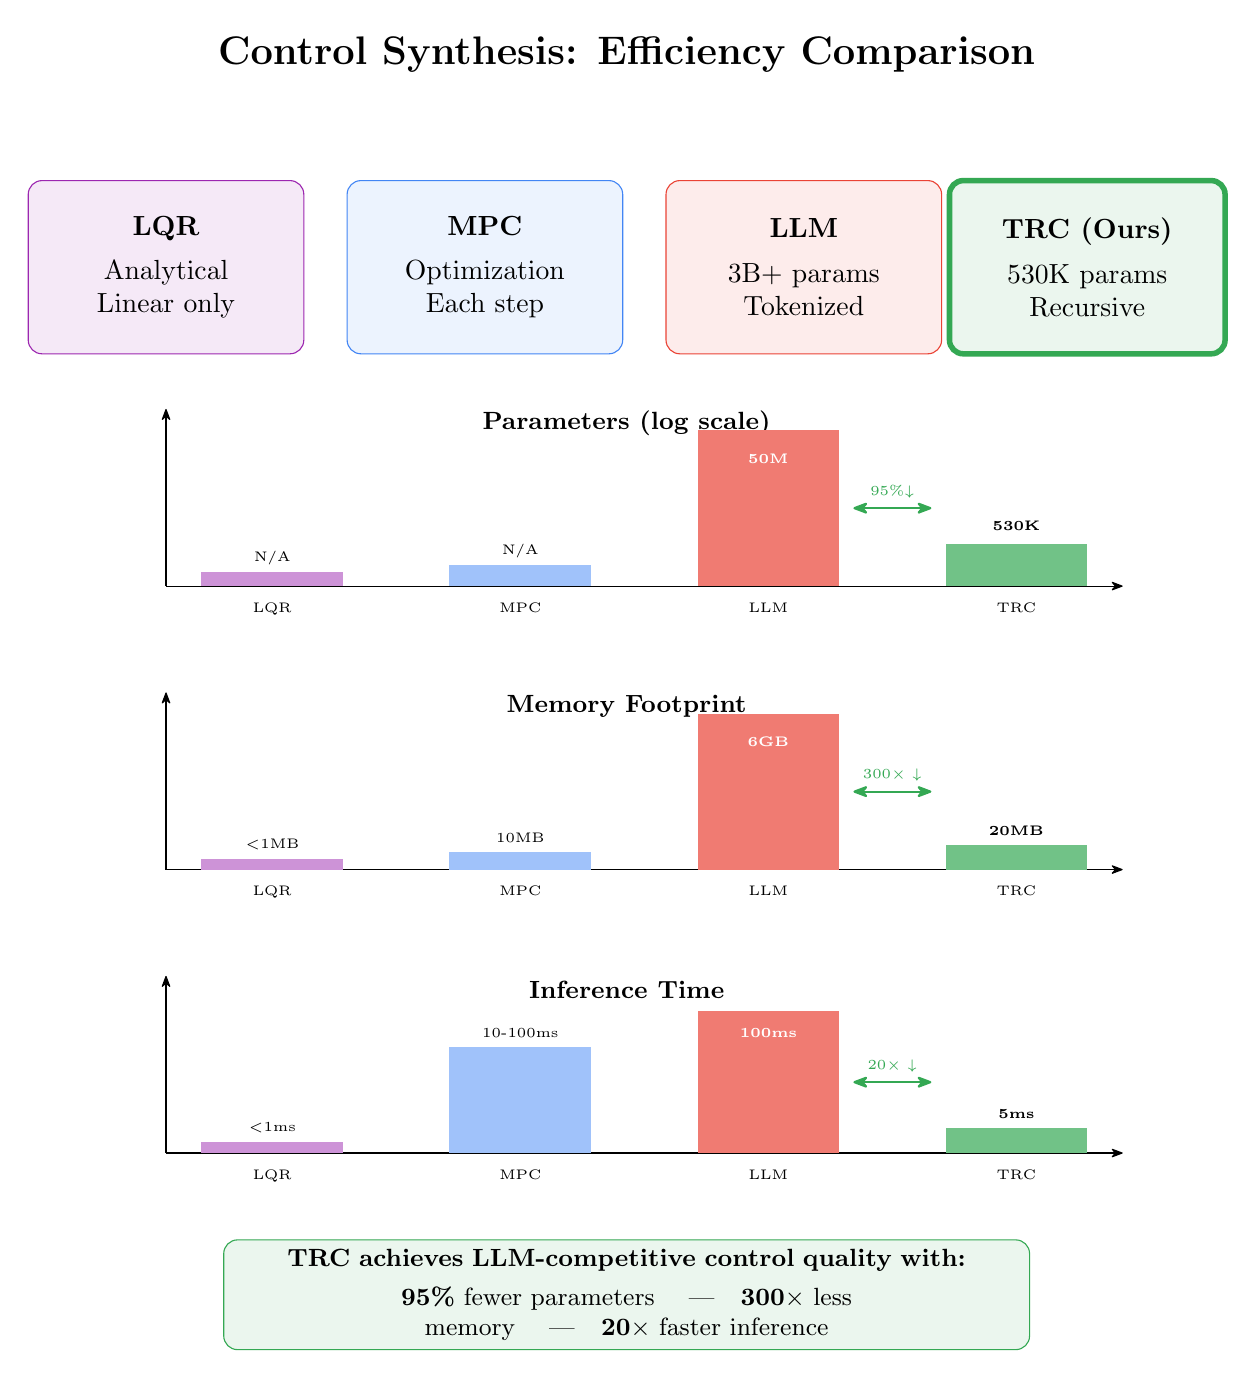
\begin{tikzpicture}[
    scale=0.9,
    >={Stealth[round]},
    method/.style={rectangle, rounded corners=5pt, draw=#1, fill=#1!10, minimum width=3.5cm, minimum height=2.2cm, align=center},
    metric/.style={font=\scriptsize},
    arrow/.style={->, thick}
]

% Title
\node[font=\Large\bfseries] at (6.5, 6) {Control Synthesis: Efficiency Comparison};

% ===================== METHODS =====================

% LQR
\node[method=lqrcolor] (lqr) at (0, 3) {
    \textbf{LQR}\\[4pt]
    \metric{Analytical}\\
    \metric{Linear only}
};

% MPC
\node[method=mpccolor] (mpc) at (4.5, 3) {
    \textbf{MPC}\\[4pt]
    \metric{Optimization}\\
    \metric{Each step}
};

% LLM
\node[method=llmcolor] (llm) at (9, 3) {
    \textbf{LLM}\\[4pt]
    \metric{3B+ params}\\
    \metric{Tokenized}
};

% TRC (highlighted)
\node[method=trccolor, line width=2pt] (trc) at (13, 3) {
    \textbf{TRC (Ours)}\\[4pt]
    \metric{530K params}\\
    \metric{Recursive}
};

% ===================== METRICS BAR CHARTS =====================

% Parameters comparison
\node[font=\small\bfseries] at (6.5, 0.8) {Parameters (log scale)};

% Bar chart
\begin{scope}[shift={(0, -1.5)}]
    % Axis
    \draw[->] (0, 0) -- (13.5, 0);
    \draw[->] (0, 0) -- (0, 2.5);

    % Labels
    \node[font=\tiny, anchor=north] at (1.5, -0.1) {LQR};
    \node[font=\tiny, anchor=north] at (5, -0.1) {MPC};
    \node[font=\tiny, anchor=north] at (8.5, -0.1) {LLM};
    \node[font=\tiny, anchor=north] at (12, -0.1) {TRC};

    % Bars (log scale visualization)
    % LQR - N/A (represented as minimal)
    \fill[lqrcolor!50] (0.5, 0) rectangle (2.5, 0.2);
    \node[font=\tiny] at (1.5, 0.4) {N/A};

    % MPC - ~1M (represented as minimal)
    \fill[mpccolor!50] (4, 0) rectangle (6, 0.3);
    \node[font=\tiny] at (5, 0.5) {N/A};

    % LLM - 50M trainable
    \fill[llmcolor!70] (7.5, 0) rectangle (9.5, 2.2);
    \node[font=\tiny, white] at (8.5, 1.8) {\textbf{50M}};

    % TRC - 530K
    \fill[trccolor!70] (11, 0) rectangle (13, 0.6);
    \node[font=\tiny] at (12, 0.85) {\textbf{530K}};

    % Annotation
    \draw[<->, thick, trccolor] (9.7, 1.1) -- (10.8, 1.1) node[midway, above, font=\tiny] {95\%$\downarrow$};
\end{scope}

% Memory comparison
\node[font=\small\bfseries] at (6.5, -3.2) {Memory Footprint};

\begin{scope}[shift={(0, -5.5)}]
    % Axis
    \draw[->] (0, 0) -- (13.5, 0);
    \draw[->] (0, 0) -- (0, 2.5);

    % Labels
    \node[font=\tiny, anchor=north] at (1.5, -0.1) {LQR};
    \node[font=\tiny, anchor=north] at (5, -0.1) {MPC};
    \node[font=\tiny, anchor=north] at (8.5, -0.1) {LLM};
    \node[font=\tiny, anchor=north] at (12, -0.1) {TRC};

    % Bars
    % LQR
    \fill[lqrcolor!50] (0.5, 0) rectangle (2.5, 0.15);
    \node[font=\tiny] at (1.5, 0.35) {$<$1MB};

    % MPC
    \fill[mpccolor!50] (4, 0) rectangle (6, 0.25);
    \node[font=\tiny] at (5, 0.45) {10MB};

    % LLM - 6GB
    \fill[llmcolor!70] (7.5, 0) rectangle (9.5, 2.2);
    \node[font=\tiny, white] at (8.5, 1.8) {\textbf{6GB}};

    % TRC - 20MB
    \fill[trccolor!70] (11, 0) rectangle (13, 0.35);
    \node[font=\tiny] at (12, 0.55) {\textbf{20MB}};

    % Annotation
    \draw[<->, thick, trccolor] (9.7, 1.1) -- (10.8, 1.1) node[midway, above, font=\tiny] {300$\times\downarrow$};
\end{scope}

% Inference time comparison
\node[font=\small\bfseries] at (6.5, -7.2) {Inference Time};

\begin{scope}[shift={(0, -9.5)}]
    % Axis
    \draw[->] (0, 0) -- (13.5, 0);
    \draw[->] (0, 0) -- (0, 2.5);

    % Labels
    \node[font=\tiny, anchor=north] at (1.5, -0.1) {LQR};
    \node[font=\tiny, anchor=north] at (5, -0.1) {MPC};
    \node[font=\tiny, anchor=north] at (8.5, -0.1) {LLM};
    \node[font=\tiny, anchor=north] at (12, -0.1) {TRC};

    % Bars
    % LQR
    \fill[lqrcolor!50] (0.5, 0) rectangle (2.5, 0.15);
    \node[font=\tiny] at (1.5, 0.35) {$<$1ms};

    % MPC - variable
    \fill[mpccolor!50] (4, 0) rectangle (6, 1.5);
    \node[font=\tiny] at (5, 1.7) {10-100ms};

    % LLM - 100ms
    \fill[llmcolor!70] (7.5, 0) rectangle (9.5, 2);
    \node[font=\tiny, white] at (8.5, 1.7) {\textbf{100ms}};

    % TRC - 5ms
    \fill[trccolor!70] (11, 0) rectangle (13, 0.35);
    \node[font=\tiny] at (12, 0.55) {\textbf{5ms}};

    % Annotation
    \draw[<->, thick, trccolor] (9.7, 1) -- (10.8, 1) node[midway, above, font=\tiny] {20$\times\downarrow$};
\end{scope}

% ===================== KEY TAKEAWAY =====================
\node[draw=trccolor, rounded corners=5pt, fill=trccolor!10, text width=10cm, align=center, font=\small] at (6.5, -11.5) {
    \textbf{TRC achieves LLM-competitive control quality with:}\\[3pt]
    \textbf{95\%} fewer parameters \quad|\quad \textbf{300$\times$} less memory \quad|\quad \textbf{20$\times$} faster inference
};

\end{tikzpicture}

\end{document}
